% Options for packages loaded elsewhere
\PassOptionsToPackage{unicode}{hyperref}
\PassOptionsToPackage{hyphens}{url}
%
\documentclass[
]{book}
\usepackage{amsmath,amssymb}
\usepackage{lmodern}
\usepackage{iftex}
\ifPDFTeX
  \usepackage[T1]{fontenc}
  \usepackage[utf8]{inputenc}
  \usepackage{textcomp} % provide euro and other symbols
\else % if luatex or xetex
  \usepackage{unicode-math}
  \defaultfontfeatures{Scale=MatchLowercase}
  \defaultfontfeatures[\rmfamily]{Ligatures=TeX,Scale=1}
\fi
% Use upquote if available, for straight quotes in verbatim environments
\IfFileExists{upquote.sty}{\usepackage{upquote}}{}
\IfFileExists{microtype.sty}{% use microtype if available
  \usepackage[]{microtype}
  \UseMicrotypeSet[protrusion]{basicmath} % disable protrusion for tt fonts
}{}
\makeatletter
\@ifundefined{KOMAClassName}{% if non-KOMA class
  \IfFileExists{parskip.sty}{%
    \usepackage{parskip}
  }{% else
    \setlength{\parindent}{0pt}
    \setlength{\parskip}{6pt plus 2pt minus 1pt}}
}{% if KOMA class
  \KOMAoptions{parskip=half}}
\makeatother
\usepackage{xcolor}
\usepackage{color}
\usepackage{fancyvrb}
\newcommand{\VerbBar}{|}
\newcommand{\VERB}{\Verb[commandchars=\\\{\}]}
\DefineVerbatimEnvironment{Highlighting}{Verbatim}{commandchars=\\\{\}}
% Add ',fontsize=\small' for more characters per line
\usepackage{framed}
\definecolor{shadecolor}{RGB}{248,248,248}
\newenvironment{Shaded}{\begin{snugshade}}{\end{snugshade}}
\newcommand{\AlertTok}[1]{\textcolor[rgb]{0.94,0.16,0.16}{#1}}
\newcommand{\AnnotationTok}[1]{\textcolor[rgb]{0.56,0.35,0.01}{\textbf{\textit{#1}}}}
\newcommand{\AttributeTok}[1]{\textcolor[rgb]{0.77,0.63,0.00}{#1}}
\newcommand{\BaseNTok}[1]{\textcolor[rgb]{0.00,0.00,0.81}{#1}}
\newcommand{\BuiltInTok}[1]{#1}
\newcommand{\CharTok}[1]{\textcolor[rgb]{0.31,0.60,0.02}{#1}}
\newcommand{\CommentTok}[1]{\textcolor[rgb]{0.56,0.35,0.01}{\textit{#1}}}
\newcommand{\CommentVarTok}[1]{\textcolor[rgb]{0.56,0.35,0.01}{\textbf{\textit{#1}}}}
\newcommand{\ConstantTok}[1]{\textcolor[rgb]{0.00,0.00,0.00}{#1}}
\newcommand{\ControlFlowTok}[1]{\textcolor[rgb]{0.13,0.29,0.53}{\textbf{#1}}}
\newcommand{\DataTypeTok}[1]{\textcolor[rgb]{0.13,0.29,0.53}{#1}}
\newcommand{\DecValTok}[1]{\textcolor[rgb]{0.00,0.00,0.81}{#1}}
\newcommand{\DocumentationTok}[1]{\textcolor[rgb]{0.56,0.35,0.01}{\textbf{\textit{#1}}}}
\newcommand{\ErrorTok}[1]{\textcolor[rgb]{0.64,0.00,0.00}{\textbf{#1}}}
\newcommand{\ExtensionTok}[1]{#1}
\newcommand{\FloatTok}[1]{\textcolor[rgb]{0.00,0.00,0.81}{#1}}
\newcommand{\FunctionTok}[1]{\textcolor[rgb]{0.00,0.00,0.00}{#1}}
\newcommand{\ImportTok}[1]{#1}
\newcommand{\InformationTok}[1]{\textcolor[rgb]{0.56,0.35,0.01}{\textbf{\textit{#1}}}}
\newcommand{\KeywordTok}[1]{\textcolor[rgb]{0.13,0.29,0.53}{\textbf{#1}}}
\newcommand{\NormalTok}[1]{#1}
\newcommand{\OperatorTok}[1]{\textcolor[rgb]{0.81,0.36,0.00}{\textbf{#1}}}
\newcommand{\OtherTok}[1]{\textcolor[rgb]{0.56,0.35,0.01}{#1}}
\newcommand{\PreprocessorTok}[1]{\textcolor[rgb]{0.56,0.35,0.01}{\textit{#1}}}
\newcommand{\RegionMarkerTok}[1]{#1}
\newcommand{\SpecialCharTok}[1]{\textcolor[rgb]{0.00,0.00,0.00}{#1}}
\newcommand{\SpecialStringTok}[1]{\textcolor[rgb]{0.31,0.60,0.02}{#1}}
\newcommand{\StringTok}[1]{\textcolor[rgb]{0.31,0.60,0.02}{#1}}
\newcommand{\VariableTok}[1]{\textcolor[rgb]{0.00,0.00,0.00}{#1}}
\newcommand{\VerbatimStringTok}[1]{\textcolor[rgb]{0.31,0.60,0.02}{#1}}
\newcommand{\WarningTok}[1]{\textcolor[rgb]{0.56,0.35,0.01}{\textbf{\textit{#1}}}}
\usepackage{longtable,booktabs,array}
\usepackage{calc} % for calculating minipage widths
% Correct order of tables after \paragraph or \subparagraph
\usepackage{etoolbox}
\makeatletter
\patchcmd\longtable{\par}{\if@noskipsec\mbox{}\fi\par}{}{}
\makeatother
% Allow footnotes in longtable head/foot
\IfFileExists{footnotehyper.sty}{\usepackage{footnotehyper}}{\usepackage{footnote}}
\makesavenoteenv{longtable}
\usepackage{graphicx}
\makeatletter
\def\maxwidth{\ifdim\Gin@nat@width>\linewidth\linewidth\else\Gin@nat@width\fi}
\def\maxheight{\ifdim\Gin@nat@height>\textheight\textheight\else\Gin@nat@height\fi}
\makeatother
% Scale images if necessary, so that they will not overflow the page
% margins by default, and it is still possible to overwrite the defaults
% using explicit options in \includegraphics[width, height, ...]{}
\setkeys{Gin}{width=\maxwidth,height=\maxheight,keepaspectratio}
% Set default figure placement to htbp
\makeatletter
\def\fps@figure{htbp}
\makeatother
\setlength{\emergencystretch}{3em} % prevent overfull lines
\providecommand{\tightlist}{%
  \setlength{\itemsep}{0pt}\setlength{\parskip}{0pt}}
\setcounter{secnumdepth}{-\maxdimen} % remove section numbering
\ifLuaTeX
  \usepackage{selnolig}  % disable illegal ligatures
\fi
\IfFileExists{bookmark.sty}{\usepackage{bookmark}}{\usepackage{hyperref}}
\IfFileExists{xurl.sty}{\usepackage{xurl}}{} % add URL line breaks if available
\urlstyle{same} % disable monospaced font for URLs
\hypersetup{
  pdftitle={The data-wrangling and omics course for R novices},
  pdfauthor={Casper-Emil Tingskov Pedersen and Jonathan Thorsen},
  hidelinks,
  pdfcreator={LaTeX via pandoc}}

\title{The data-wrangling and omics course for R novices}
\author{Casper-Emil Tingskov Pedersen and Jonathan Thorsen}
\date{2023-11-03}

\begin{document}
\frontmatter
\maketitle

\mainmatter
\hypertarget{welcome}{%
\chapter{Welcome to this course}\label{welcome}}


\includegraphics[width=0.85\textwidth,height=\textheight]{Data_analyses2.jpeg}

This course will introduce you to data-wrangling and analysis of omics
data. We start out by building an intuition for working with data in
R/Rstudio and then plot our results.

The best way to learn is to follow along with your own laptop, but all
are welcome. The idea with this course is also that you can do your own
selv-paced learning by going back to themes that are harder.

We'll spend half the time with the lectures on the basic of R and data
wrangling and half the time for you to try out wrangling yourself. You
can also try some of the things you learn from the exercises on your own
data.

Before you begin, be sure you are all set up: see the prerequisites in
\#overview.

Breakdown for the course:

\begin{center}\rule{0.5\linewidth}{0.5pt}\end{center}

\textbf{Course schedule:}

\begin{longtable}[]{@{}
  >{\raggedright\arraybackslash}p{(\columnwidth - 4\tabcolsep) * \real{0.1084}}
  >{\raggedright\arraybackslash}p{(\columnwidth - 4\tabcolsep) * \real{0.4940}}
  >{\raggedright\arraybackslash}p{(\columnwidth - 4\tabcolsep) * \real{0.3976}}@{}}
\toprule()
\begin{minipage}[b]{\linewidth}\raggedright
Time
\end{minipage} & \begin{minipage}[b]{\linewidth}\raggedright
Day1
\end{minipage} & \begin{minipage}[b]{\linewidth}\raggedright
Day2
\end{minipage} \\
\midrule()
\endhead
9-10:30 & Data-Wrangling, an introduction & Modelling introduction and
omics \\
10:35-12 & Get your hands dirty with data-wrangling & Your own catwalk
with omics \\
13-14.30 & GGplot2, an introduction & Machine learning introduction \\
14.35-16 & Plotting visually please plots & Omics and machine
learning \\
\bottomrule()
\end{longtable}

\begin{center}\rule{0.5\linewidth}{0.5pt}\end{center}

This work is licensed under a
\href{https://creativecommons.org/licenses/by/4.0/}{Creative Commons
Attribution 4.0 International License}.

\hypertarget{overview}{%
\chapter{Course overview}\label{overview}}

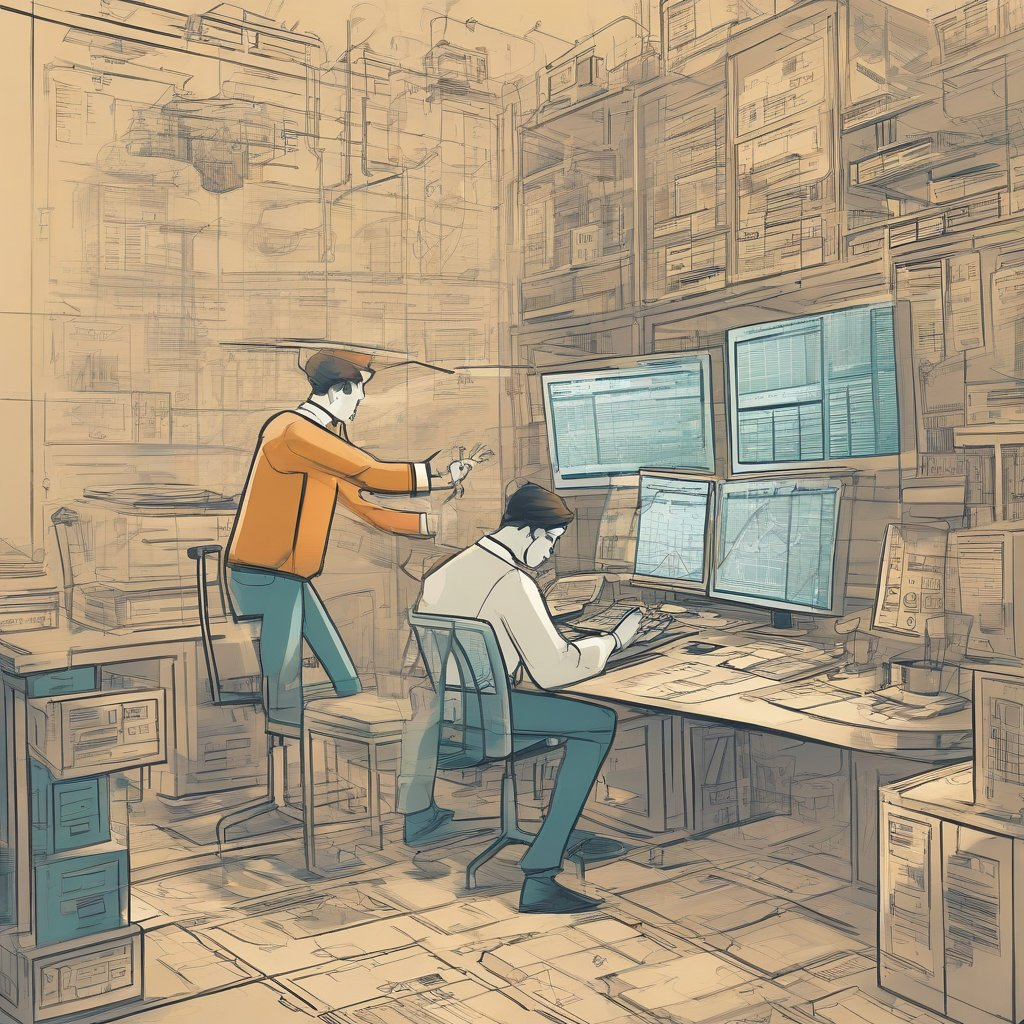
\includegraphics[width=0.75\textwidth,height=\textheight]{Data_wrangling1.jpeg}

Yihaa you are commited to learning relevant coding using R. The world is
now ready to become your oister.

\hypertarget{what-can-you-expect}{%
\section{What can you expect}\label{what-can-you-expect}}

In this course you will learn how to code in R and it will be fun. You
will learn efficient code and workflows that can be used in your own
research and for various kinds of data, including all types of omics
data. This is really powerful and will lead you to become a better
scientist.

\hypertarget{general-learning-outcomes}{%
\section{General learning outcomes}\label{general-learning-outcomes}}

-how to code in R.

-how to THINK about data.

-how to think about data separately from your research questions.

-how and why to tidy data and analyze tidy data.

-how to increase efficiency in your research.

\hypertarget{our-workflow-plus-the-tidy-data-workflow}{%
\section{Our workflow plus the Tidy data
workflow}\label{our-workflow-plus-the-tidy-data-workflow}}

We will turning our data tidy and how to use a tidyverse suite of tools
to work with tidy data.\\
It has been developed by \href{https://hadley.nz/}{Hadley Wickham} and
his team, please visit his website if you are interested in learning
more.

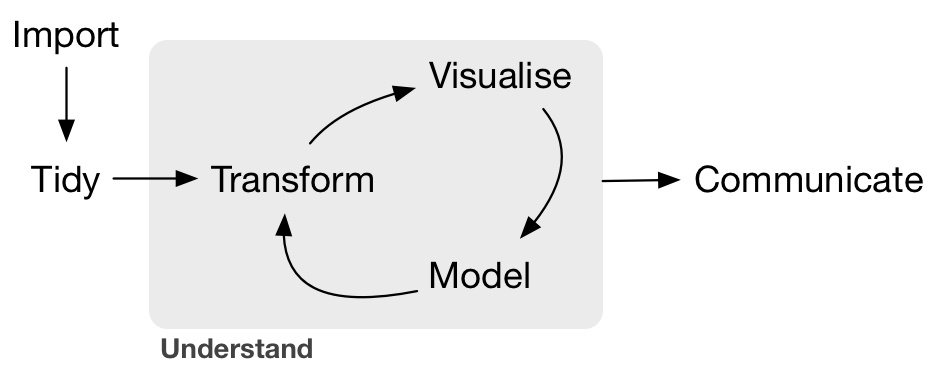
\includegraphics{https://ohi-science.org/data-science-training/img/r4ds_data-science.png}

We will be focusing on a combination of tools:

Basic tools: -\textbf{str/glimpse}: Look at data

Tidytools:

-\textbf{Tidy}: \texttt{tidyr} to organize rows of data into unique
values.

-\textbf{Transform}: \texttt{dplyr} to manipulate/wrangle data based on
subsetting by rows or columns, sorting and joining.

-\textbf{Visualize}: \texttt{ggplot2} static plots, using grammar of
graphics principles

This is essential - Instead of building your analyses around the format
your data are in, take deliberate steps to make your data tidy. When
your data are tidy, you can use a growing suite of powerful analytical
and visualization tools instead of inventing home-grown ways to
accommodate your data. This will save you time since you aren't
reinventing the wheel, and will make your work more clear and
understandable to your collaborators (most importantly, Future You).

\hypertarget{working-with-data-that-is-not-your-own}{%
\section{Working with data that is not your
own}\label{working-with-data-that-is-not-your-own}}

One of the most important things you will learn is how to think about
data separately from your own research context. Said in another way,
you'll learn to distinguish your data questions from your research
questions. Here, we are focusing on data questions, and we will use data
that is not specific to your research.

We will be using several different data sets throughout this training,
and will help you see the patterns and parallels to your own data, which
will ultimately help you in your research.

\hypertarget{goals-of-this-course}{%
\section{Goals of this course}\label{goals-of-this-course}}

The goal of this course today is to equip you with the tools to take a
(your) dataset and do the following:

\begin{enumerate}
\def\labelenumi{\arabic{enumi}.}
\tightlist
\item
  Import data to R and understand the structure of your data
\item
  Look at it using summaries and descriptive statistics
\item
  Engineer features relevant for your research
\item
  Impute missing data
\item
  To do transformation and understand what that means
\item
  Plot the data using visually appealing and publish-ready figures
\end{enumerate}

\hypertarget{prerequisites}{%
\section{Prerequisites}\label{prerequisites}}

A few things need to be checked before we start. First, we assume that
you have either \href{https://cloud.r-project.org/}{R} or
\href{https://www.rstudio.com/products/rstudio/download/}{RStudio}
installed.

Also, if not already installed, please install the following packages:
c(``dplyr'',``tidyverse'',``broom'',``\,``)

\hypertarget{credit}{%
\section{Credit}\label{credit}}

This material builds from (and is directly copied from) a lot of
fantastic materials developed by others in the open data science
community. In particular, it pulls from the following resources, which
are highly recommended for further learning and as resources later on.
Specific lessons will also cite more resources.

\href{https://ohi-science.org/data-science-training/overview.html}{OHI
data science training}

\href{https://moderndive.netlify.app/1-getting-started}{Modern dive}

\hypertarget{dataintro}{%
\chapter{Super quick intro to coding and data in R}\label{dataintro}}


\includegraphics[width=0.75\textwidth,height=\textheight]{Data_analyses.jpeg}

\hypertarget{codingprogramming-in-r}{%
\section{Coding/programming in R}\label{codingprogramming-in-r}}

Now that you're set up with R and RStudio, you are probably asking
yourself, ``OK. Now how do I use R?''. The first thing to note is that
unlike other statistical software programs like Excel, SPSS, or Minitab
that provide point-and-click interfaces, R is an interpreted language.
This means you have to type in commands written in R code. In other
words, you have to code/program in R. Note that we'll use the terms
``coding'' and ``programming'' interchangeably throughout this course.

While it is not required to be a seasoned coder/computer programmer to
use R, there is still a set of basic programming concepts that new R
users need to understand. Consequently, while this course is not focused
on learning programming, you will still learn just enough of these basic
programming concepts needed to explore and analyze data effectively.

\hypertarget{basic-terminology-in-r}{%
\section{Basic terminology in R}\label{basic-terminology-in-r}}

We now introduce some basic programming concepts and terminology.
Instead of asking you to memorize all these concepts and terminology
right now, we'll guide you so that you'll ``learn by doing.'' To help
you learn, we will always use a different font to distinguish regular
text from computer\_code. Also we will go through a tiny bit of
information and then ask you do a similar task on your computer.

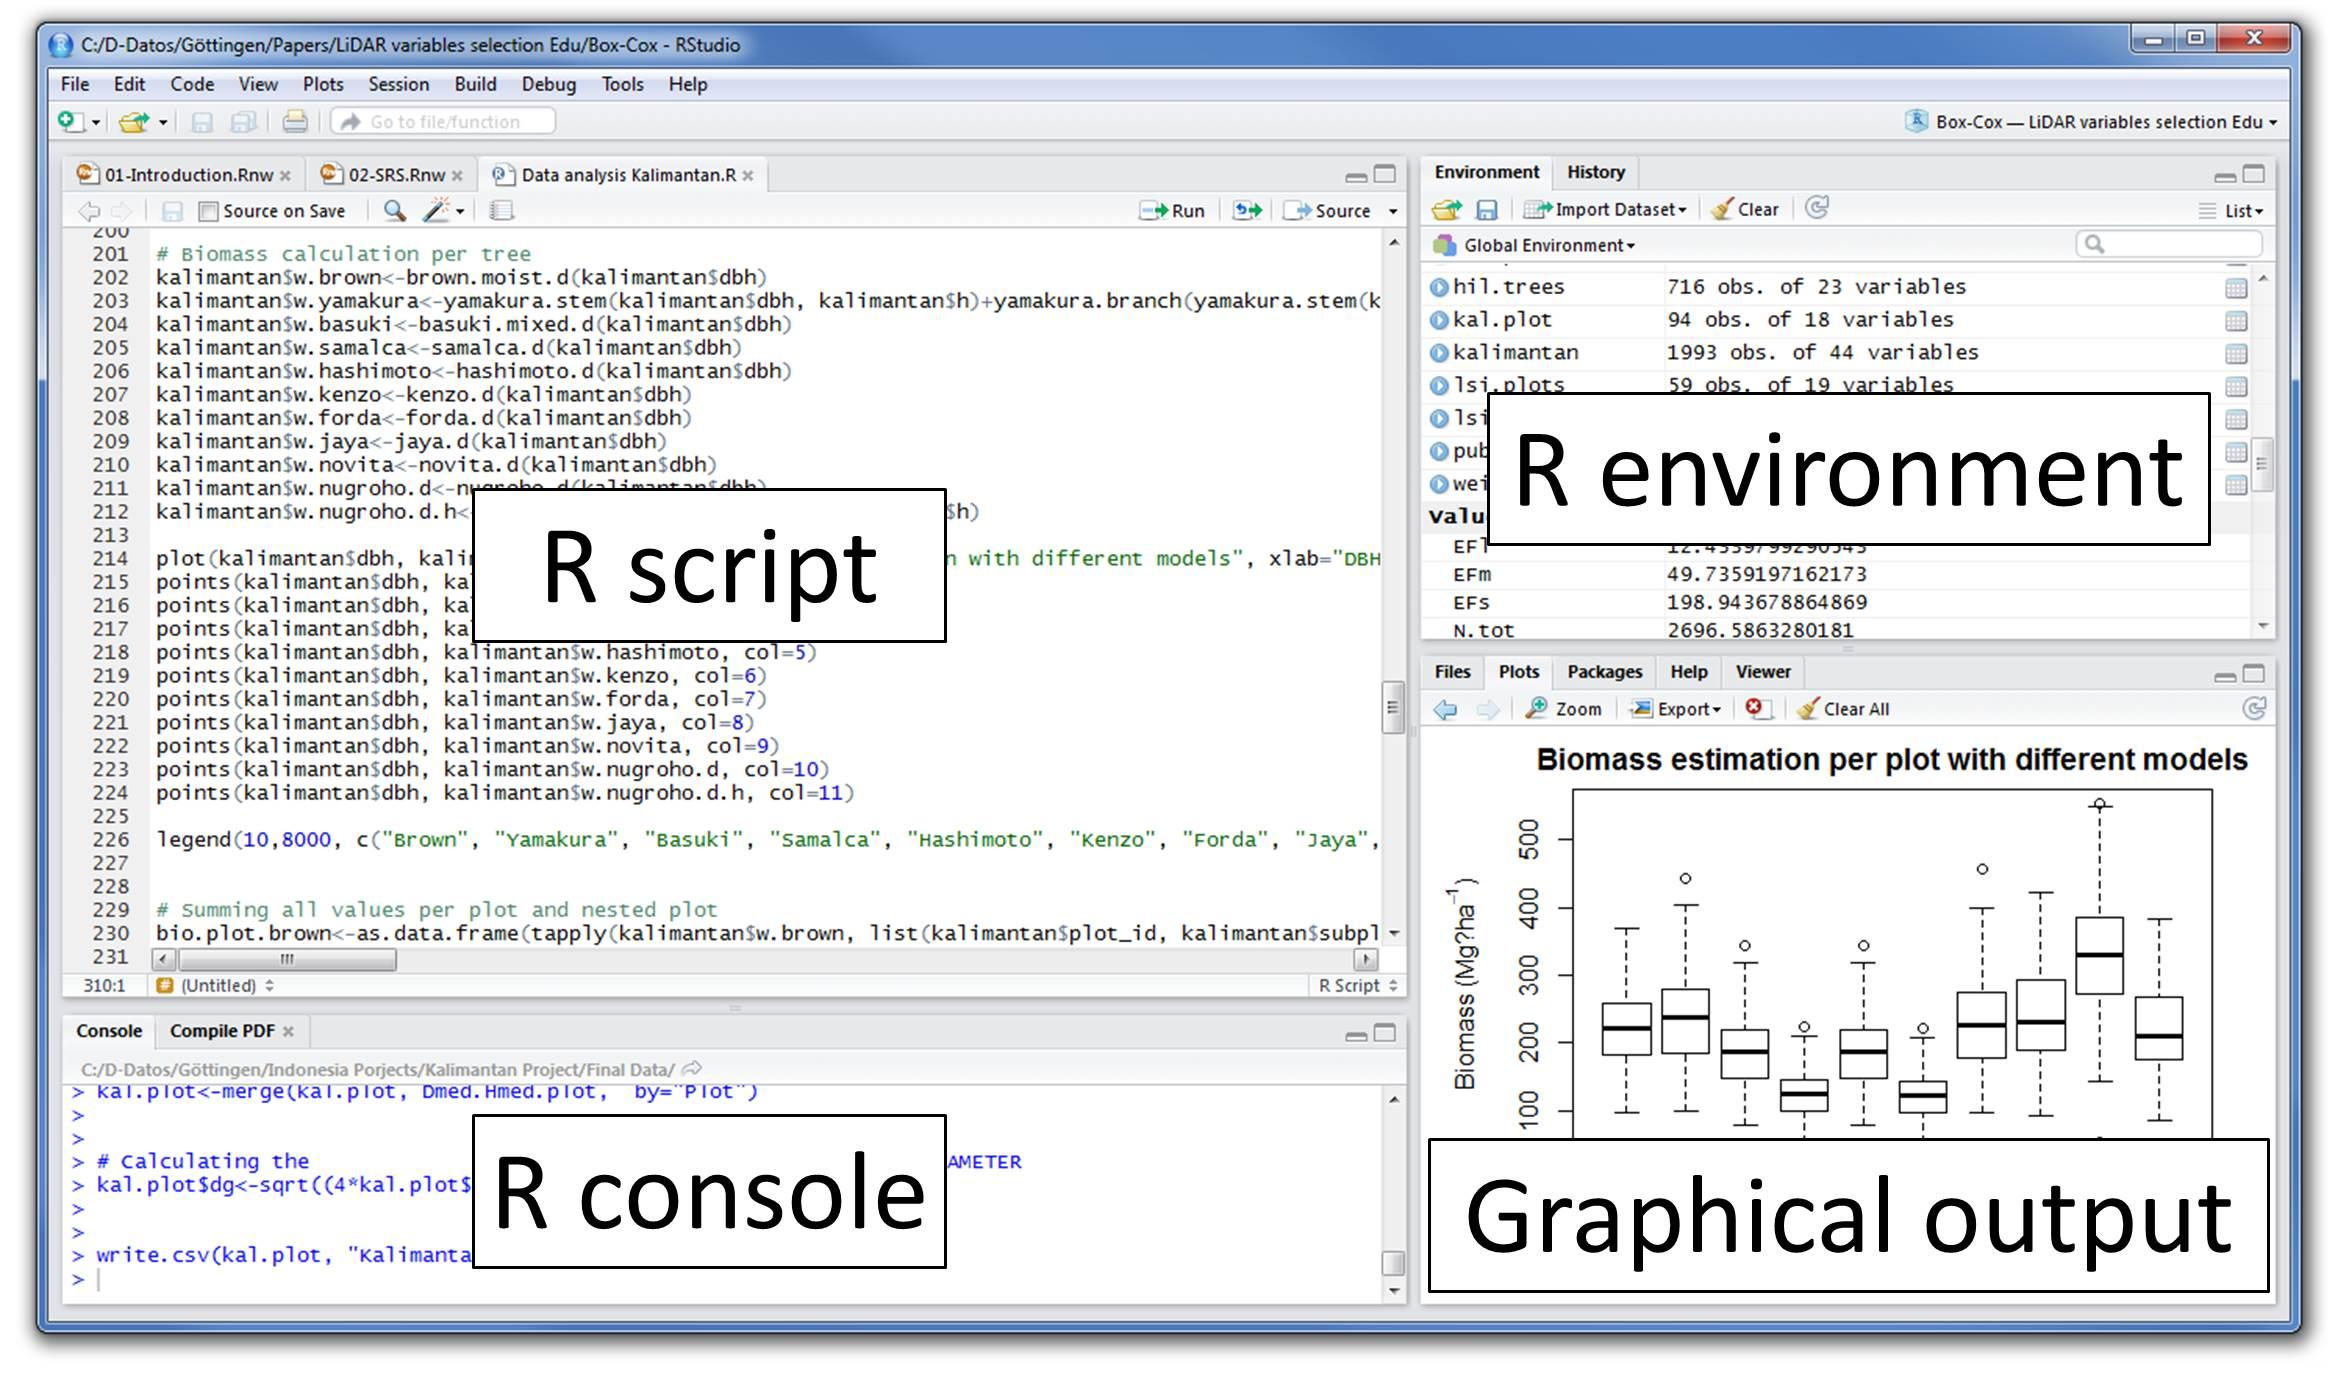
\includegraphics{https://www.analyticsvidhya.com/wp-content/uploads/2016/02/rstudio.jpg}

On this plot you can see the overview of Rstudio. This contains the
following elements:

Console pane: where you enter in commands.

R script: Where you store your commands often in a text file.

R environment: What objects are registered/loaded in the environment (we
will get back to that).

Graphical output: Where you can see figures that is produced by commands
in the console.

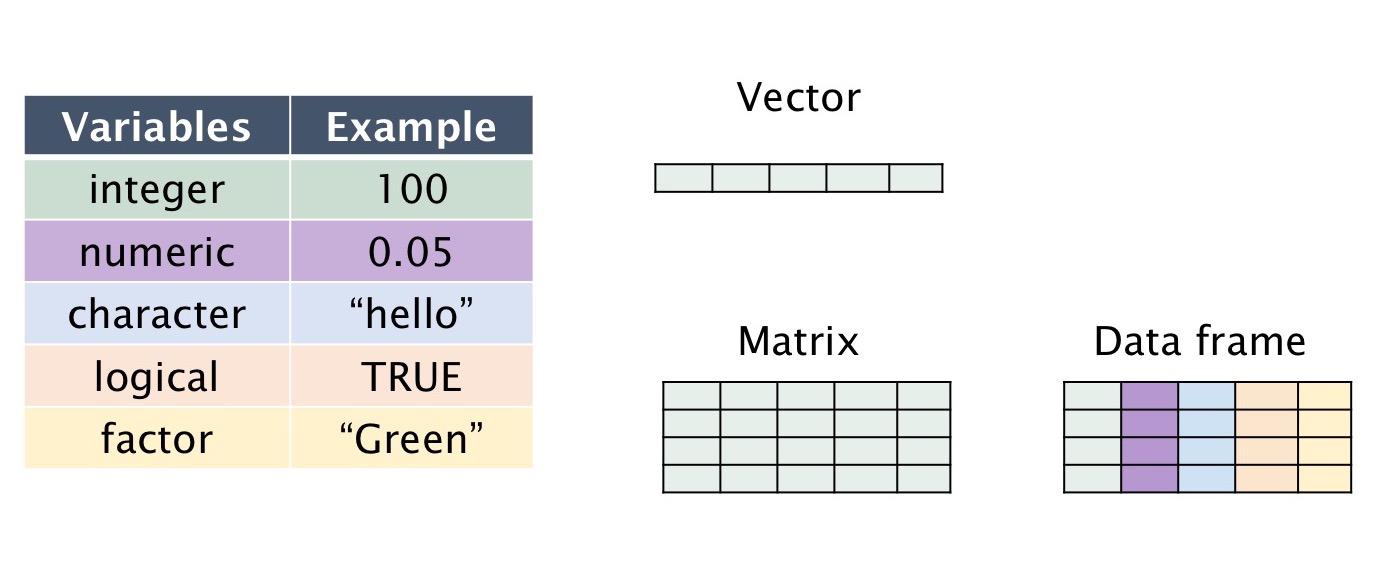
\includegraphics{https://sydney-informatics-hub.github.io/lessonbmc/fig/Rvariablesdata.jpg}

This figure shows some of the more important data types in R and how
they relate to storing data in R. It seems simple when set up like this,
but when you are coding and you need to find an error this figure is a
good place to start.

Vectors can be created by using the \texttt{c()} function in R. The c
stands for concatenate. for example the following command creates a
vector of integers 1,2,3,4:
\texttt{my\_vector\ \textless{}-\ c(1,2,3,4)}

Matrices can be created by using the \texttt{matrix()} function in R.
Matrices are great for doing calculations incredibly fast BUT they can
only contain one type of data unlike dataframes. For example the
following command creates a matrix with the same four integers 1,2,3,4:
\texttt{my\_matrix\ \textless{}-\ matrix(c(1,2,3,4))} you can also
rearrange the matrix so that it has two columns instead of one:
\texttt{my\_matrix\ \textless{}-\ matrix(c(1,2,3,4),ncol=2)} you can
look at your matrix by typing \texttt{my\_matrix} in the console.

Data frames is a way to store data containing both strings, integers,
factors together. They are rectangular spreadsheets. Typically you have
a dataset where the rows correspond tot eh observations/samples and the
columns correspond to the variables that describe the observations. And
this is the typical format when we analyse data. We can create a data
frame in R with mixed data like this:
\texttt{my\_df\ \textless{}-\ data.frame(int\ =\ c(1,2,3,4),names\ =\ c("Villy","Søren","Karl","Benny"))}.

\includegraphics{https://help.displayr.com/hc/article_attachments/6719912862607}

\emph{Conditionals:}

Often we subset our data using conditions, e.g.~we only want samples of
our data frame that has a value in column 3 that is larger than X. Do
this kind of subsetting, we use \emph{conditionals}.

For example, using the data frame from before, we can restrict rows to
those that have a integer value larger than 2 like this:
\texttt{my\_df{[}my\_df\$int\ \textgreater{}\ 2,{]}} This will capture
the last two rows of the data. Notice the comma, which is essential when
indexing dataframes: everything before the comma is subsetting on rows
while after the comma is for subsetting columns. We can also subset
using equality using == (and NOT =, which is used for assignment). Here
is an example using equality:
\texttt{my\_df{[}my\_df\$names\ ==\ "Karl",{]}}.\\
The final example of something similar to but not identical is a binary
operator \%in\% which is not listed in the figure above but still very
useful. This weirdly looking \%in\% is describing a operator (which we
will get back to and use later) which can search for overlaps e.g.~in R:
\texttt{my\_df{[}my\_df\$names\ \%in\%\ c("Karl","Villy"),{]}} See here
that we find the overlap between names in my\_df and the provided vector
and only showing the rows of the data frame where there is an overlap.

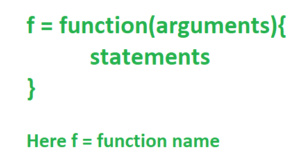
\includegraphics{https://media.geeksforgeeks.org/wp-content/uploads/20200411225124/f114-300x158.png}

Functions, also called commands: Functions perform tasks in R. They take
in inputs called arguments and return outputs. You can either manually
specify a function's arguments or use the function's default values. For
example, the function \texttt{seq()} in R generates a sequence of
numbers. If you just run \texttt{seq()} it will return the value 1. That
doesn't seem very useful! This is because the default arguments are set
as \texttt{seq(from\ =\ 1,\ to\ =\ 1)}. Thus, if you don't pass in
different values for from and to to change this behavior, R just assumes
all you want is the number 1. You can change the argument values by
updating the values after the = sign. If we try out
\texttt{seq(from\ =\ 2,\ to\ =\ 5)} we get the result 2 3 4 5 that we
might expect.

This list is by no means an exhaustive list of all the programming
concepts and terminology needed to become a savvy R user; such a list
would be so large it wouldn't be very useful, especially for novices.
Rather, we feel this is a minimally viable list of programming concepts
and terminology you need to know before getting started. We feel that
you can learn the rest as you go. Remember that your mastery of all of
these concepts and terminology will build as you practice more and more.

\hypertarget{exercise1}{%
\subsection{Your turn}\label{exercise1}}

Exercise 1.

\begin{enumerate}
\def\labelenumi{\arabic{enumi}.}
\item
  Create a dataframe with the following information (you pick the
  dataframe name): two column dataframe. One with the names:
  \texttt{c("Villy","Søren","Karl","Benny","Siri")} and One with the
  following grades:\texttt{c(100,20,40,30,60)}.
\item
  Use the \texttt{mean()} function to calculate the mean for passing
  grades (\textgreater30). There are many ways to do this but a hint is
  that we only need to run one command. you can always see more
  information about the function by writing \texttt{?mean} in your
  console.
\end{enumerate}

\hypertarget{error-messages}{%
\section{Error messages}\label{error-messages}}

One thing that intimidates new R and RStudio users is how it reports
errors, warnings, and messages. R reports errors, warnings, and messages
in a glaring red font, which makes it seem like it is scolding you.
However, seeing red text in the console is not always bad.

R will show red text in the console pane in three different situations:

\includegraphics{https://media.wired.com/photos/593257829be5e55af6c24476/master/w_2240,c_limit/trafficlight-inline.jpg}

If the text starts with ``Error'', figure out what's causing it. Think
of errors as a red traffic light: something is wrong! If the text starts
with ``Warning'', figure out if it's something to worry about. For
instance, if you get a warning about missing values in a scatterplot and
you know there are missing values, you're fine. If that's surprising,
look at your data and see what's missing. Think of warnings as a yellow
traffic light: everything is working fine, but watch out/pay attention.
Otherwise, the text is just a message. Read it, wave back at R, and
thank it for talking to you. Think of messages as a green traffic light:
everything is working fine and keep on going!

\hypertarget{coding-tips-and-tricks}{%
\section{Coding tips and tricks}\label{coding-tips-and-tricks}}

Learning to code/program is quite similar to learning a foreign
language. It can be daunting and frustrating at first. Such frustrations
are common and it is normal to feel discouraged as you learn. However,
just as with learning a foreign language, if you put in the effort and
are not afraid to make mistakes, anybody can learn and improve.

Here are a few useful tips to keep in mind as you learn to program:

\includegraphics{https://cdn.vox-cdn.com/thumbor/BKeBuV-Agjw4SaAA8Mbm1ptN7e0=/0x0:4032x3024/620x465/filters:focal(1693x1446:2337x2090):format(webp)/cdn.vox-cdn.com/uploads/chorus_image/image/59740845/sip_of_joy.17.jpg}

\emph{Remember that computers are not actually that smart}: You may
think your computer or smartphone is ``smart,'' but really people spent
a lot of time and energy designing them to appear ``smart.'' In reality,
you have to tell a computer everything it needs to do. Furthermore, the
instructions you give your computer can't have any mistakes in them, nor
can they be ambiguous in any way.

\emph{Take the ``copy, paste, and tweak'' approach}: Especially when you
learn your first programming language or you need to understand
particularly complicated code, it is often much easier to take existing
code that you know works and modify it to suit your ends. This is as
opposed to trying to type out the code from scratch. We call this the
``copy, paste, and tweak'' approach. So early on, we suggest not trying
to write code from memory, but rather take existing examples we have
provided you, then copy, paste, and tweak them to suit your goals. After
you start feeling more confident, you can slowly move away from this
approach and write code from scratch. Think of the ``copy, paste, and
tweak'' approach as training wheels for a child learning to ride a bike.
After getting comfortable, they won't need them anymore.

\emph{The best way to learn to code is by doing:} Rather than learning
to code for its own sake, we find that learning to code goes much
smoother when you have a goal in mind or when you are working on a
particular project, like analyzing data that you are interested in and
that is important to you.\\
Practice is key!

\hypertarget{installpackages}{%
\section{Install and load package}\label{installpackages}}

So we alluded to that the environment contains many objects and some of
these objects come from packages. Packages in R is precalculated
functions and useful tools to work with your data. Therefore, embrace
packages and get familiar with some of them. Some of the more important
ones we will use in this course are: \texttt{tidyverse} and
\texttt{dplyr} for data massaging and wrangling and \texttt{ggplot\ 2}
for visualizations.

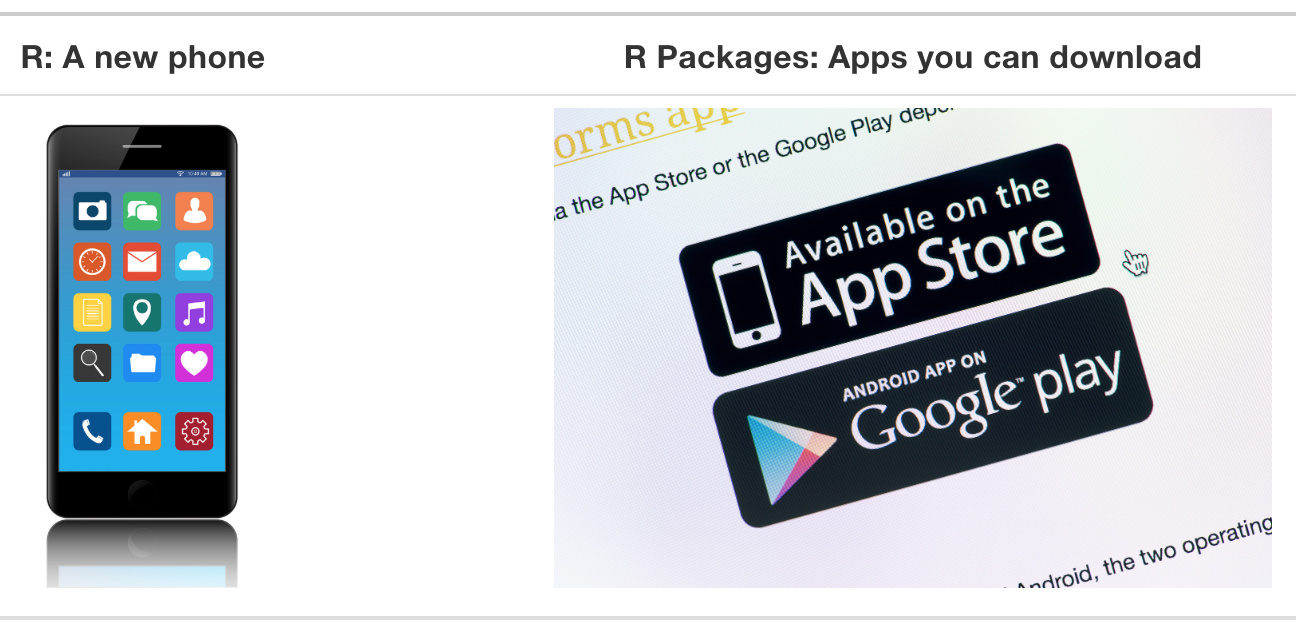
\includegraphics{https://moderndive.netlify.app/images/shutterstock/R_vs_R_packages.png}

So R is like a new mobile phone: while it has a certain amount of
features when you use it for the first time, it doesn't have everything.
R packages are like the apps you can download onto your phone from
Apple's App Store or Android's Google Play.

Like an app on your smartphone, you need to install it first and the
open it.

if you try to load a package that is not installed you get an error for
instance

\texttt{library(tidyverse)} and if not you know that tidyverse is
installed

To install the tidyverse package do the following:

\texttt{install.packages("tidyverse")}

and to load it subsequently, write \texttt{library(tidyverse)}.

Now install \texttt{broom} , \texttt{tidyverse} and \texttt{dplyr} using
this approach

\hypertarget{datawrangling}{%
\chapter{Data wrangling and tidy data}\label{datawrangling}}

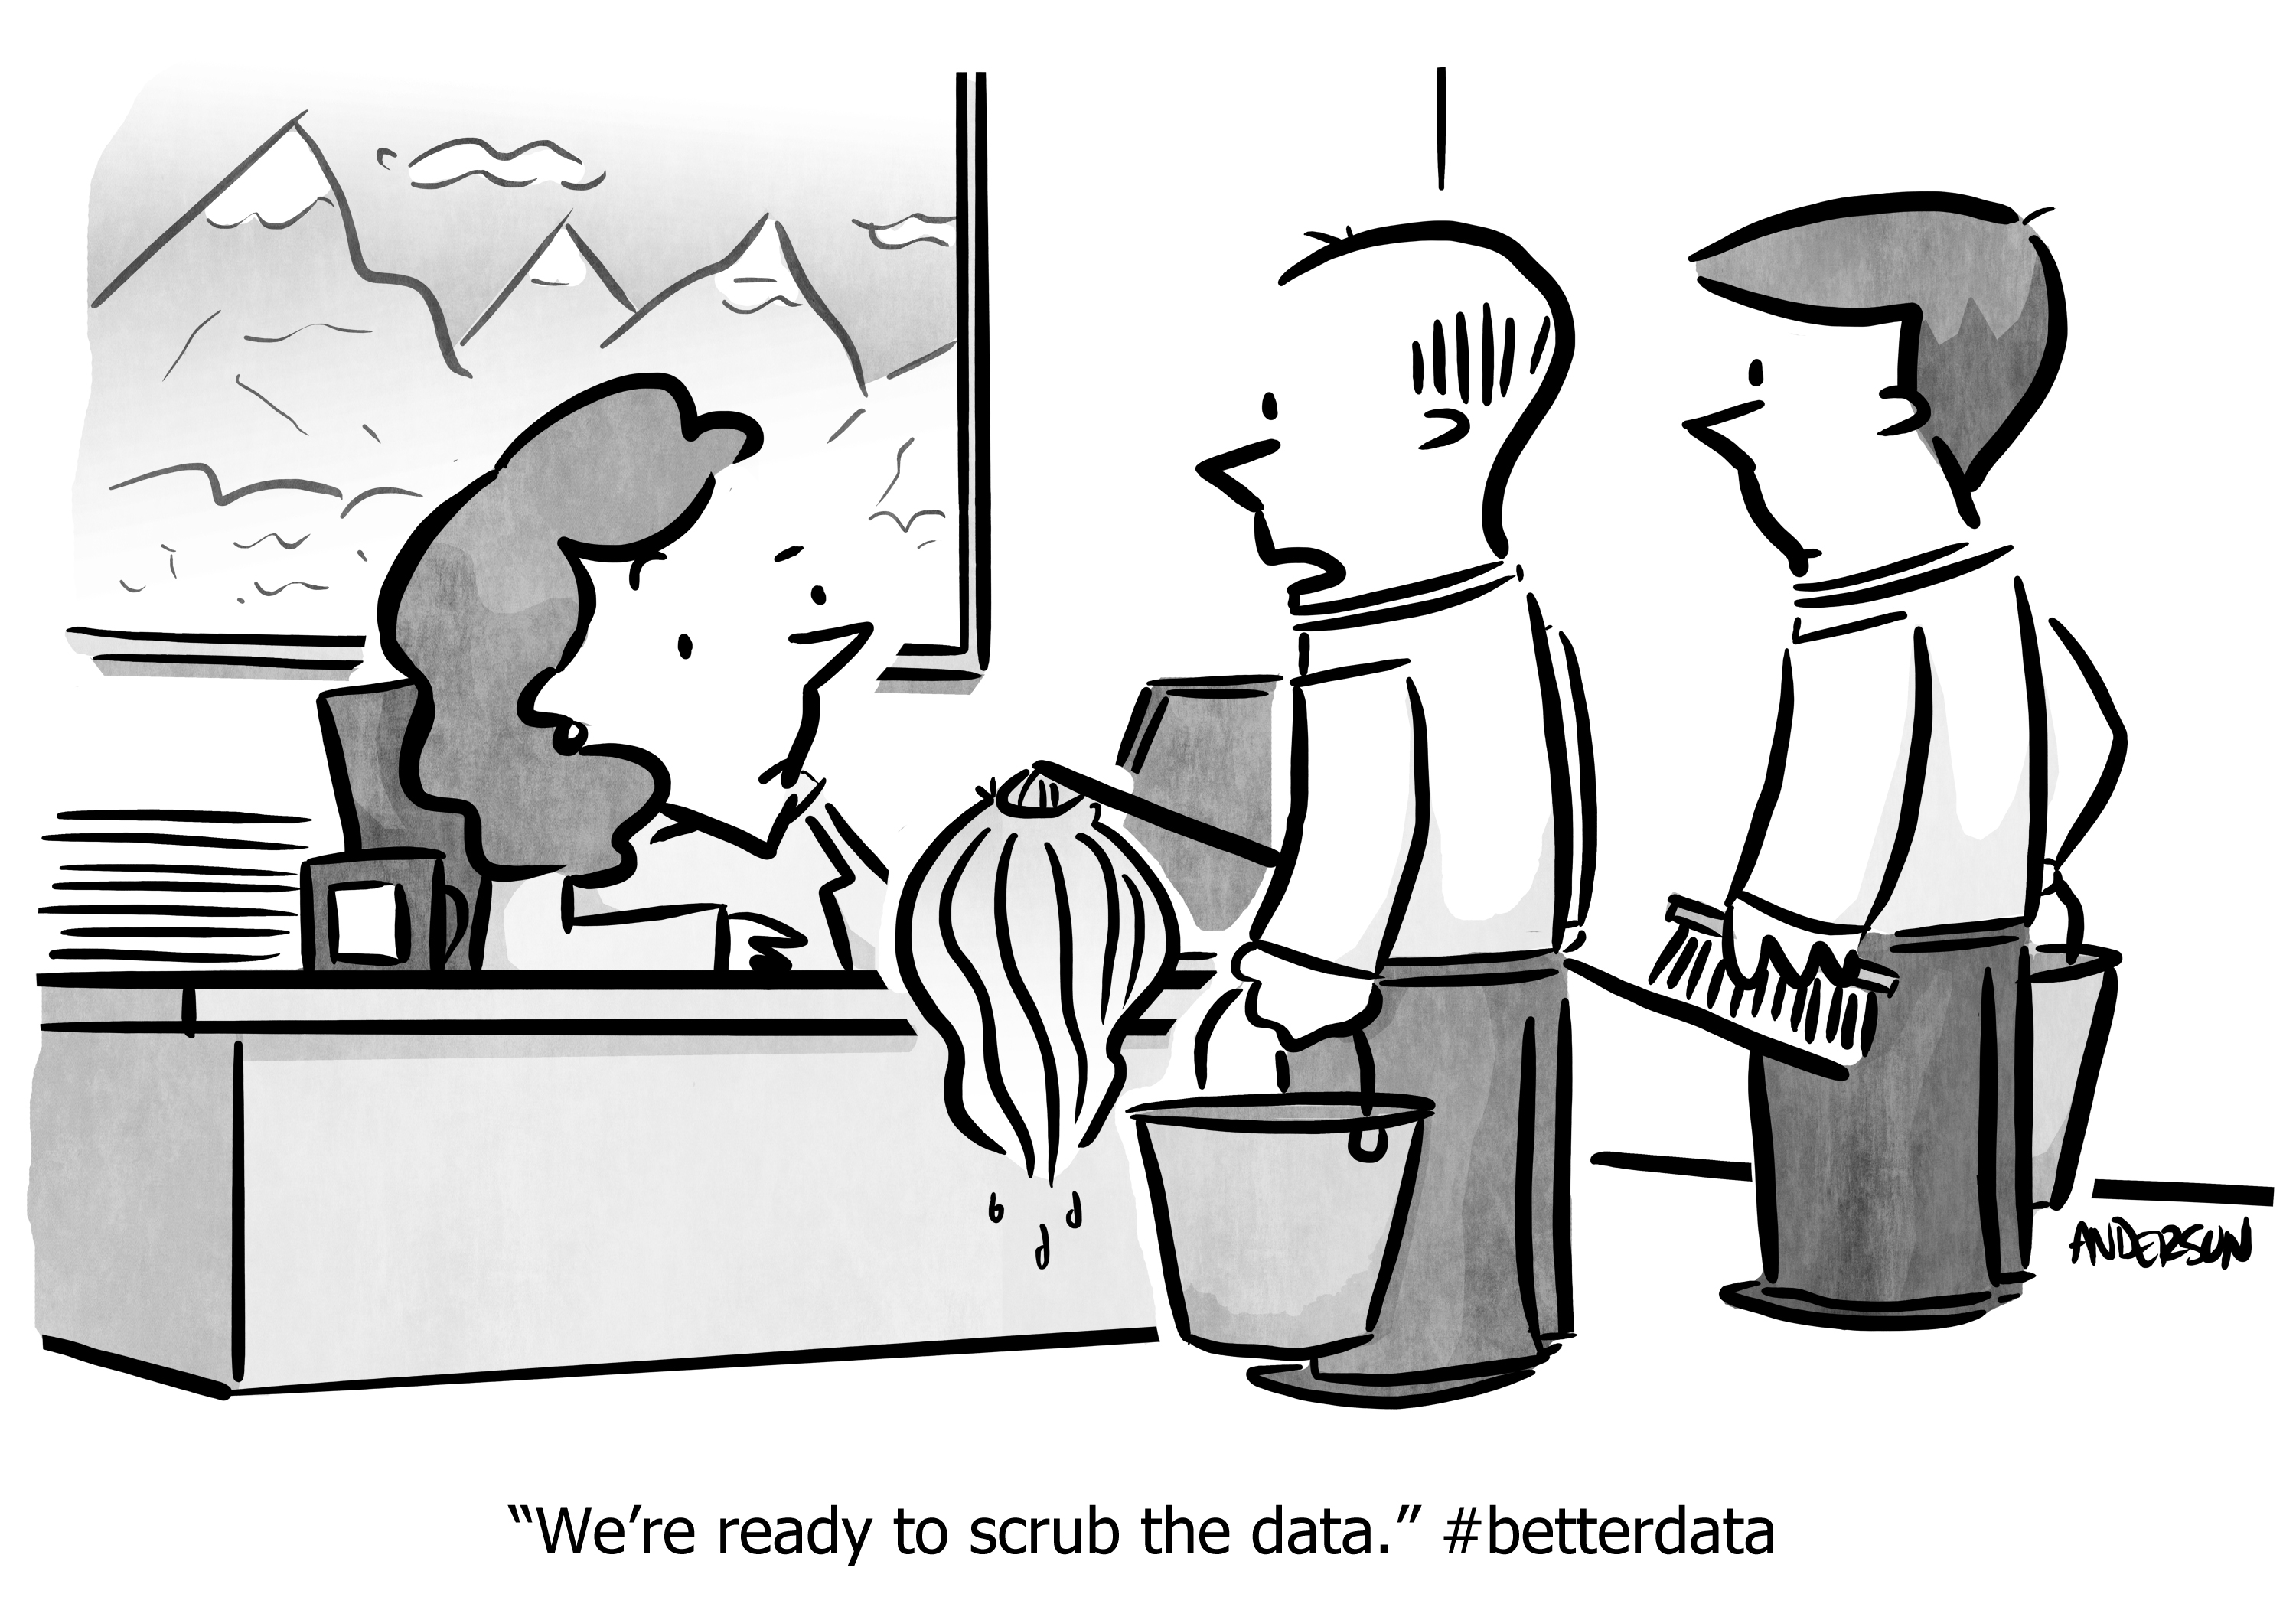
\includegraphics{https://andreashandel.github.io/MADAcourse/media/cartoonscrubdata.jpg}

\hypertarget{packages-required}{%
\section{Packages required}\label{packages-required}}

The following packages are required. If you need to go back and check
how installing a package is done see the section 3.5(\#installpackages).

library(dplyr).\\
library(ggplot2).\\
library(readr).\\
library(tidyr).\\
library(broom).\\
library(palmerpenguins).

This chapter will introduce you to data wrangling with an emphasis on
the \texttt{dplyr} package along with other helpful functions. You will
see how powerful wrangling can be and how it can be like a magic wand to
transform data into your specific needs. The key functions include but
are not limited to:

\begin{enumerate}
\def\labelenumi{\arabic{enumi}.}
\item
  The overarching function which makes us able to combine functions and
  subsetting is \textbf{the pipe}. And what is a pipe? Pipes are a neat
  way to tie together several dataframes/functions into a chain of
  actions. It makes coding easier to understand and is therefore a
  better style of coding. It looks like this
  \texttt{\%\textgreater{}\%}. For instance taking the mean of the first
  two rows of the \texttt{my\_df} dataframe can be done like so:
  \texttt{my\_df{[}1:2,"Grades"{]}\ \%\textgreater{}\%\ mean}. Learning
  to use the pipe to your advantage is learning to code. Luckily it all
  comes naturally when working with the following functions:
\item
  \texttt{left\_join()} merge two data frames together using a key
  column. This function (along with its cousin functions
  \texttt{right\_join()} and \texttt{join()} etc.) is the bread and
  butter of working with many data types that needs to be merged and
  analysed. For example
\end{enumerate}

\begin{Shaded}
\begin{Highlighting}[]
  \FunctionTok{library}\NormalTok{(dplyr) }
\NormalTok{  my\_data }\OtherTok{\textless{}{-}} \FunctionTok{data.frame}\NormalTok{(}
  \AttributeTok{names =} \FunctionTok{c}\NormalTok{(}\StringTok{"Villy"}\NormalTok{, }\StringTok{"Søren"}\NormalTok{, }\StringTok{"Karl"}\NormalTok{, }\StringTok{"Benny"}\NormalTok{, }\StringTok{"Siri"}\NormalTok{),}
  \AttributeTok{Grades =} \FunctionTok{c}\NormalTok{(}\DecValTok{100}\NormalTok{, }\DecValTok{20}\NormalTok{, }\DecValTok{40}\NormalTok{, }\DecValTok{30}\NormalTok{, }\DecValTok{60}\NormalTok{),}
  \AttributeTok{gender =} \FunctionTok{c}\NormalTok{(}\StringTok{"boy"}\NormalTok{, }\StringTok{"boy"}\NormalTok{, }\StringTok{"boy"}\NormalTok{, }\StringTok{"boy"}\NormalTok{, }\StringTok{"girl"}\NormalTok{)) }
\NormalTok{  other\_data }\OtherTok{\textless{}{-}} \FunctionTok{data.frame}\NormalTok{(}\AttributeTok{gender =} \FunctionTok{c}\NormalTok{(}\StringTok{"boy"}\NormalTok{, }\StringTok{"girl"}\NormalTok{), }\AttributeTok{description =} \FunctionTok{c}\NormalTok{(}\StringTok{"Male"}\NormalTok{, }\StringTok{"Female"}\NormalTok{))}
\NormalTok{  left\_joined\_data }\OtherTok{\textless{}{-}} \FunctionTok{left\_join}\NormalTok{(my\_data, other\_data, }\AttributeTok{by =} \StringTok{"gender"}\NormalTok{) }
  
\NormalTok{  left\_joined\_data}
\end{Highlighting}
\end{Shaded}

\begin{verbatim}
##   names Grades gender description
## 1 Villy    100    boy        Male
## 2 Søren     20    boy        Male
## 3  Karl     40    boy        Male
## 4 Benny     30    boy        Male
## 5  Siri     60   girl      Female
\end{verbatim}

\begin{enumerate}
\def\labelenumi{\arabic{enumi}.}
\tightlist
\item
  \texttt{mutate()} construct/reconstruct a column using a newly defined
  column name. This function is useful to generate a new columns that
  modify existing ones often using a conditional to do so. Now using the
  same data as above:
\end{enumerate}

\begin{Shaded}
\begin{Highlighting}[]
\NormalTok{  mutated\_data }\OtherTok{\textless{}{-}}\NormalTok{ my\_data }\SpecialCharTok{\%\textgreater{}\%}
  \FunctionTok{mutate}\NormalTok{(}\AttributeTok{Grades\_scaled =}\NormalTok{ Grades }\SpecialCharTok{/} \FunctionTok{max}\NormalTok{(Grades))}
\end{Highlighting}
\end{Shaded}

\begin{enumerate}
\def\labelenumi{\arabic{enumi}.}
\tightlist
\item
  \texttt{glimpse()} take a sneak peak at a dataset. Useful for getting
  the dimensions of the data and the type of data contained in the
  columns. Now look at the newly constructed column
\end{enumerate}

\begin{Shaded}
\begin{Highlighting}[]
  \FunctionTok{glimpse}\NormalTok{(mutated\_data)}
\end{Highlighting}
\end{Shaded}

\begin{verbatim}
## Rows: 5
## Columns: 4
## $ names         <chr> "Villy", "Søren", "Karl", "Benny", "Siri"
## $ Grades        <dbl> 100, 20, 40, 30, 60
## $ gender        <chr> "boy", "boy", "boy", "boy", "girl"
## $ Grades_scaled <dbl> 1.0, 0.2, 0.4, 0.3, 0.6
\end{verbatim}

\begin{enumerate}
\def\labelenumi{\arabic{enumi}.}
\tightlist
\item
  \texttt{count()} counts the n of each unique value in a column.
  Usefull to combine with mutate to see the counts of the newly
  constructed column.
\end{enumerate}

\begin{Shaded}
\begin{Highlighting}[]
\NormalTok{  counted\_data }\OtherTok{\textless{}{-}} \FunctionTok{count}\NormalTok{(my\_data, gender)}
\NormalTok{  counted\_data}
\end{Highlighting}
\end{Shaded}

\begin{verbatim}
##   gender n
## 1    boy 4
## 2   girl 1
\end{verbatim}

\begin{enumerate}
\def\labelenumi{\arabic{enumi}.}
\tightlist
\item
  \texttt{arrange()} reorder the rows of a dataframe. For example, sort
  the rows of a dataset in descending order of the column height.
\end{enumerate}

\begin{Shaded}
\begin{Highlighting}[]
\NormalTok{arranged\_data }\OtherTok{\textless{}{-}} \FunctionTok{arrange}\NormalTok{(my\_data, }\FunctionTok{desc}\NormalTok{(Grades))}
\NormalTok{arranged\_data}
\end{Highlighting}
\end{Shaded}

\begin{verbatim}
##   names Grades gender
## 1 Villy    100    boy
## 2  Siri     60   girl
## 3  Karl     40    boy
## 4 Benny     30    boy
## 5 Søren     20    boy
\end{verbatim}

\begin{enumerate}
\def\labelenumi{\arabic{enumi}.}
\item
  \texttt{select()} select columns using indexing or strings.
  e.g.~\texttt{my\_df\ \%\textgreater{}\%\ select("names")}.
\item
  \texttt{filter()} the rows of a dataframe based on a filter,
  e.g.~thresholds. It is similar to the example shown in the
  introduction, where we used old school filtering on my\_df dataframe
  \texttt{my\_df{[}my\_df\$names\ \%in\%\ c("Karl","Villy"),{]}}. Using
  the filter function and pipes you can do it like this:
  \texttt{my\_df\ \%\textgreater{}\%\ filter(names\ \%in\%\ c("Karl","Villy"))}.
\item
  \texttt{summarise()} a dataframe using one or more of its
  columns/variables with a summary statistic. Such examples could be the
  median or the mean and an example look like this:
  \texttt{my\_df\ \%\textgreater{}\%\ summarise(mean\ =\ mean(Grades))}.
  This function can be very powerful when combined with the
  \texttt{group\_by} function.
\item
  \texttt{group\_by()} is a dplyr way of grouping rows, it is a way to
  assign different rows to a group and do statistical reporting on every
  specific group in the data set. An example require us to add a third
  column to \texttt{my\_df} like this:
  \texttt{my\_df\ \textless{}-\ my\_df\ \%\textgreater{}\%\ mutate(gender\ =\ c("boy","boy","boy","boy","girl"))}.
  Now using this new \texttt{my\_df} we can \texttt{group\_by} on the
  gender column and calculate the median on this group:
\end{enumerate}

\begin{Shaded}
\begin{Highlighting}[]
\NormalTok{my\_df }\SpecialCharTok{\%\textgreater{}\%} 
  \FunctionTok{group\_by}\NormalTok{(gender) }\SpecialCharTok{\%\textgreater{}\%} 
  \FunctionTok{summarise}\NormalTok{(}\FunctionTok{median}\NormalTok{(Grades)) }
\end{Highlighting}
\end{Shaded}

\begin{verbatim}
## # A tibble: 2 x 2
##   gender `median(Grades)`
##   <chr>             <dbl>
## 1 boy                  35
## 2 girl                 60
\end{verbatim}

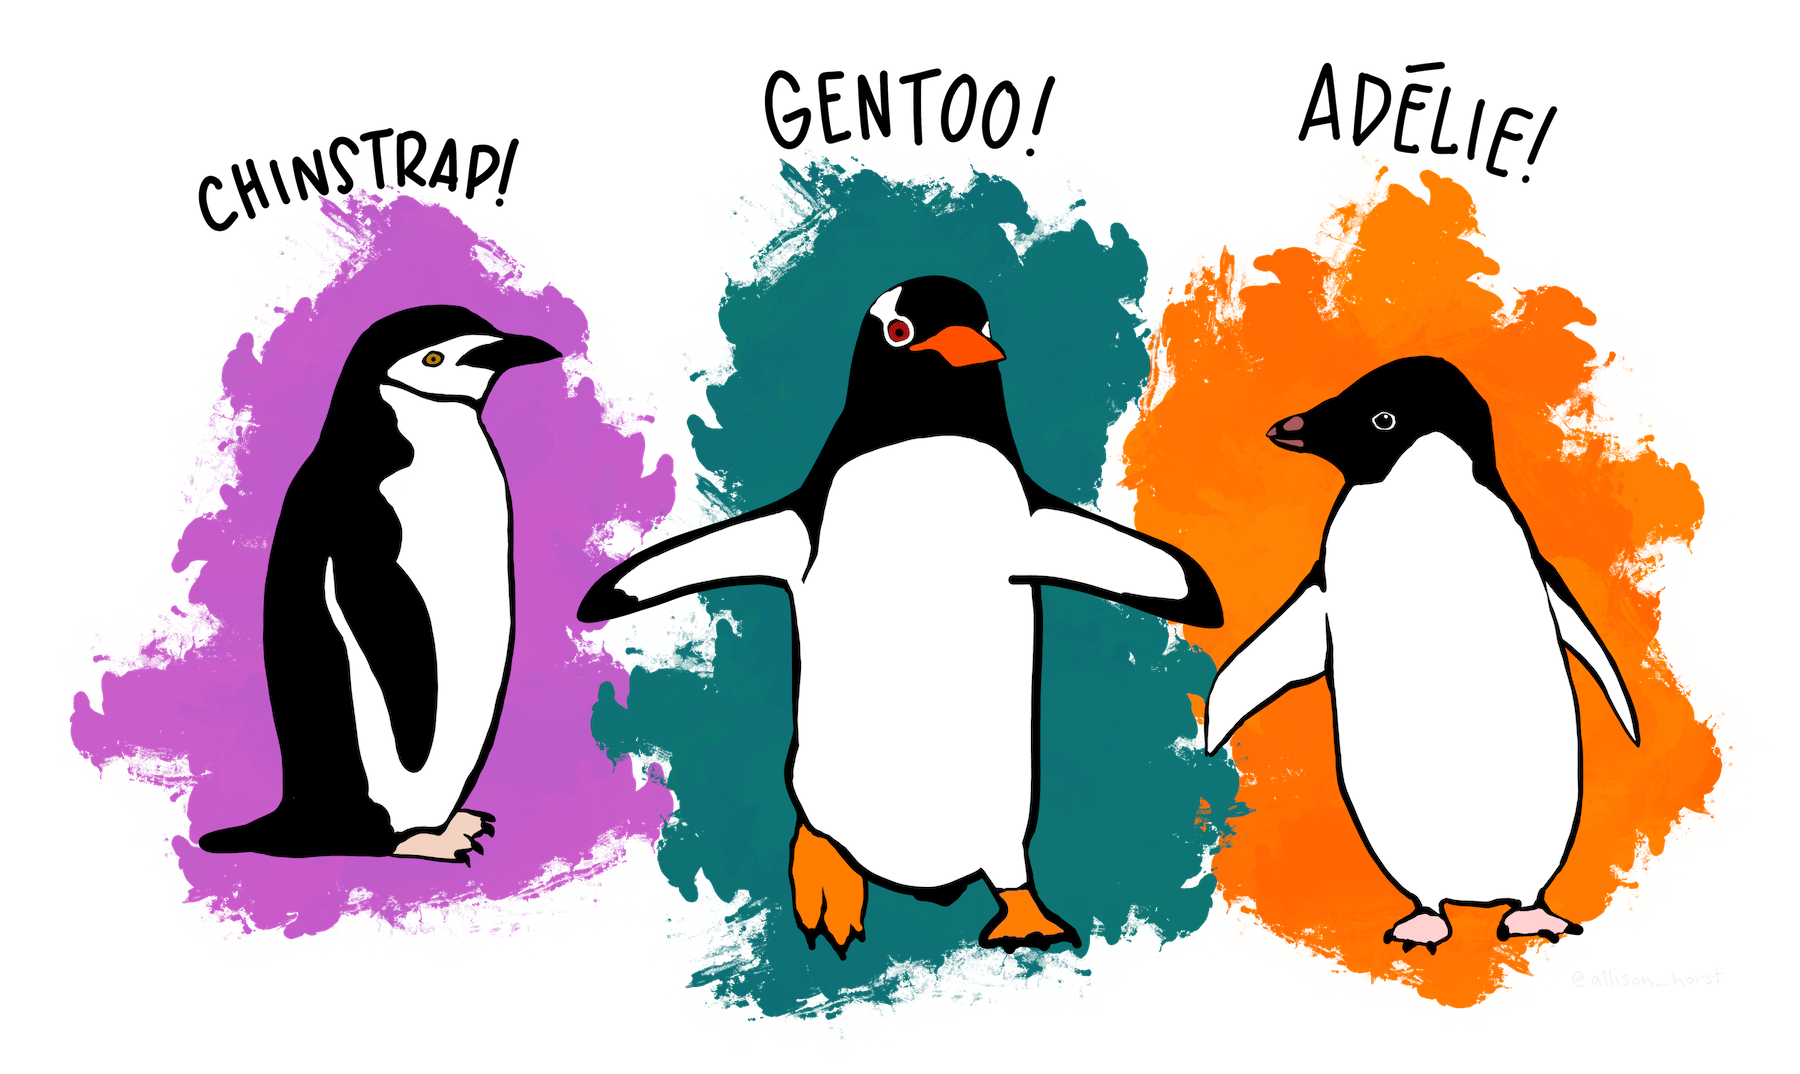
\includegraphics{https://allisonhorst.github.io/palmerpenguins/reference/figures/lter_penguins.png}

\hypertarget{penguins}{%
\section{Penguins!}\label{penguins}}

Now we are going to use the functions described above on the penguin
dataset. The data has been collected by
\href{https://gormankb.github.io/}{Dr.~Kirstin Gorman} at the Palmer
station, Antartica LTER. So real data collected for a purpose and
published in a scientific journal.

\texttt{library(palmerpenguins)}

\hypertarget{your-turn---look-at-the-dataset}{%
\subsection{Your turn - Look at the
dataset}\label{your-turn---look-at-the-dataset}}

Now look at the dataset using \texttt{glimpse()} in the console, now try
to look at the dataset using \texttt{str()} again you get information
about the dataset. Please use one minute and compare the two methods to
look at structure of the data. Which one do you prefer and why?

Exercise 2.

\begin{enumerate}
\def\labelenumi{\arabic{enumi}.}
\tightlist
\item
  You can input several grouping variables into
  \texttt{group\_by(var1,var2)}. Now use this information to output the
  mean length of the flippers for species across islands, meaning for
  e.g.~Adelie penguins you will have three values. Remember that
  \texttt{mean} can handle NA values in your dataset, you just have to
  tell it to do so.
\end{enumerate}

\hypertarget{more-handy-functions}{%
\section{More handy functions}\label{more-handy-functions}}

Often, we are interested in a summary of information for many columns at
once and thus we are not only looking at e.g.~flipper\_length across
species and islands, but rather all measurements across species and
islands. The reason to this more thorough data description is to gain
better insight into the dataset. Better insights leads to better
scientific questions.

\begin{enumerate}
\def\labelenumi{\arabic{enumi}.}
\tightlist
\item
  \texttt{across()} is a function that makes it easy to
  transform/summarise multiple columns. It needs a \emph{function} to
  apply to these columns, that could be \texttt{median} or
  \texttt{mean()}. Also, it is often combined with functions like
  \texttt{mutate()} and \texttt{summarise()} to generate new columns
  using transformation on existing columns. Furthermore, it is also
  often combined with functions that informs \texttt{across()} on which
  columns to look at. For instance, \texttt{across()} can be combined
  with \texttt{starts\_with()} and \texttt{where()}. OK enough text, now
  to an example that makes sense. Again looking at the penguins dataset,
  lets try to combine these functions to get an intuition about how they
  work together:
\end{enumerate}

\begin{Shaded}
\begin{Highlighting}[]
\NormalTok{  penguins }\SpecialCharTok{\%\textgreater{}\%} 
  \FunctionTok{group\_by}\NormalTok{(species,island) }\SpecialCharTok{\%\textgreater{}\%} 
  \FunctionTok{summarize}\NormalTok{(}\FunctionTok{across}\NormalTok{(}\FunctionTok{starts\_with}\NormalTok{(}\StringTok{"bill"}\NormalTok{),}\SpecialCharTok{\textasciitilde{}}\FunctionTok{mean}\NormalTok{(., }\AttributeTok{na.rm =} \ConstantTok{TRUE}\NormalTok{)))}
\end{Highlighting}
\end{Shaded}

\begin{verbatim}
## `summarise()` has grouped output by 'species'. You can override using the
## `.groups` argument.
\end{verbatim}

\begin{verbatim}
## # A tibble: 5 x 4
## # Groups:   species [3]
##   species   island    bill_length_mm bill_depth_mm
##   <fct>     <fct>              <dbl>         <dbl>
## 1 Adelie    Biscoe              39.0          18.4
## 2 Adelie    Dream               38.5          18.3
## 3 Adelie    Torgersen           39.0          18.4
## 4 Chinstrap Dream               48.8          18.4
## 5 Gentoo    Biscoe              47.5          15.0
\end{verbatim}

You can see that this gives a nice overview of the bill lengths across
the species across the islands. One takeaway one this would be that the
difference in bill length seems less influenced by islands and more
influenced by species.

\hypertarget{one-way-to-deal-with-missing-values}{%
\section{One way to deal with missing
values}\label{one-way-to-deal-with-missing-values}}

\begin{Shaded}
\begin{Highlighting}[]
\NormalTok{data }\OtherTok{\textless{}{-}}\NormalTok{ penguins}
\FunctionTok{sum}\NormalTok{(}\FunctionTok{is.na}\NormalTok{(penguins))}
\end{Highlighting}
\end{Shaded}

\begin{verbatim}
## [1] 19
\end{verbatim}

The penguins dataset is not perfect. BUT, we can wave our magic data
wand to impute the missing values. What is imputation? it is best-guess
construction, meaning we already know a lot about the penguins so we
fill in the missing values with guesses. It is not cheating, it is done
all the time in research.

\begin{Shaded}
\begin{Highlighting}[]
\CommentTok{\# rename the dataset so we can modify the data frame without having to reload the data}
\NormalTok{data }\OtherTok{\textless{}{-}}\NormalTok{ penguins}
\CommentTok{\# how many missing in the flipper length?}
\FunctionTok{sum}\NormalTok{(}\FunctionTok{is.na}\NormalTok{(data}\SpecialCharTok{$}\NormalTok{flipper\_length\_mm))}
\end{Highlighting}
\end{Shaded}

\begin{verbatim}
## [1] 2
\end{verbatim}

Now - waving the magic data wand - we impute

\begin{Shaded}
\begin{Highlighting}[]
\CommentTok{\# Impute missing values with mean imputation for the \textquotesingle{}flipper\_length\_mm\textquotesingle{} column}
\NormalTok{data\_imputed }\OtherTok{\textless{}{-}}\NormalTok{ data }\SpecialCharTok{\%\textgreater{}\%}
  \FunctionTok{mutate}\NormalTok{(}\AttributeTok{flipper\_length\_mm =} \FunctionTok{ifelse}\NormalTok{(}\FunctionTok{is.na}\NormalTok{(flipper\_length\_mm), }
                                    \FunctionTok{mean}\NormalTok{(flipper\_length\_mm, }\AttributeTok{na.rm =} \ConstantTok{TRUE}\NormalTok{), }
\NormalTok{                                    flipper\_length\_mm))}
\end{Highlighting}
\end{Shaded}

What is going on? Here we are being aided by the \texttt{ifelse}
function which ask questions about the data, we pair this function with
mutate and reconstruct the flipper\_length\_mm imputing missing values.

Typically though, we have a lot of variables that needs to be imputed
and \emph{even though we hate to admit it, we know that we are lazy, and
laziness is the super fuel of the efficient programmer!} So below is a
way to to the same, but instead of focusing on a specific column we use
the \texttt{mutate\_if} function to find all numeric columns in the
dataset and do the same.

\begin{Shaded}
\begin{Highlighting}[]
  \CommentTok{\# Impute missing values with mean imputation for numeric columns}
\NormalTok{  data\_imputed }\OtherTok{\textless{}{-}}\NormalTok{ data }\SpecialCharTok{\%\textgreater{}\%}
    \FunctionTok{mutate\_if}\NormalTok{(is.numeric, }\SpecialCharTok{\textasciitilde{}}\FunctionTok{ifelse}\NormalTok{(}\FunctionTok{is.na}\NormalTok{(.), }\FunctionTok{mean}\NormalTok{(., }\AttributeTok{na.rm =} \ConstantTok{TRUE}\NormalTok{), .))}
\end{Highlighting}
\end{Shaded}

\hypertarget{your-turn}{%
\subsection{Your turn}\label{your-turn}}

Exercise 3.

Sometimes the variables you need impute are not just continuous
variables like height or flipper length in mm. So what do we do then?
Well, we guess, but instead of using the information in the column you
want to impute, you use supplementary information in the adjacent
columns. How can we do that? Well consider the column in the penguins
data set which contains the gender of the penguins. We would not gain
anything from replacing NA values with the mean of that column. In the
natural world, species are often sexually dimorphic, which are fancy
words for differences in size/color between sexes. We want to leverage
this information to guess at the gender. So we can guess based on body
size because we know sexes often differ in size. But first, we need to
check if that is true for penguins.

\begin{enumerate}
\def\labelenumi{\arabic{enumi}.}
\tightlist
\item
  So assuming you have the data set called \textbf{data\_imputed} made
  above where all the continuous measurements have been mean imputed you
  can address the missing sex problem for the \emph{Adelie} species.
\end{enumerate}

Maybe you can learn something about sexual dimorphism from these plot
and table?

\begin{Shaded}
\begin{Highlighting}[]
  \FunctionTok{table}\NormalTok{(}\FunctionTok{is.na}\NormalTok{(data\_imputed}\SpecialCharTok{$}\NormalTok{sex),data\_imputed}\SpecialCharTok{$}\NormalTok{species)  }
\end{Highlighting}
\end{Shaded}

\begin{verbatim}
##        
##         Adelie Chinstrap Gentoo
##   FALSE    146        68    119
##   TRUE       6         0      5
\end{verbatim}

\begin{Shaded}
\begin{Highlighting}[]
  \FunctionTok{ggplot}\NormalTok{(data\_imputed }\SpecialCharTok{\%\textgreater{}\%} \FunctionTok{filter}\NormalTok{(species }\SpecialCharTok{\%in\%} \StringTok{"Adelie"}\NormalTok{), }\FunctionTok{aes}\NormalTok{(}\AttributeTok{x =}\NormalTok{ body\_mass\_g, }\AttributeTok{y =}\NormalTok{ flipper\_length\_mm, }\AttributeTok{color =}\NormalTok{ sex)) }\SpecialCharTok{+}
  \FunctionTok{geom\_point}\NormalTok{() }\SpecialCharTok{+}
  \FunctionTok{labs}\NormalTok{(}\AttributeTok{title =} \StringTok{"Body mass vs. flipper length by species"}\NormalTok{)}
\end{Highlighting}
\end{Shaded}

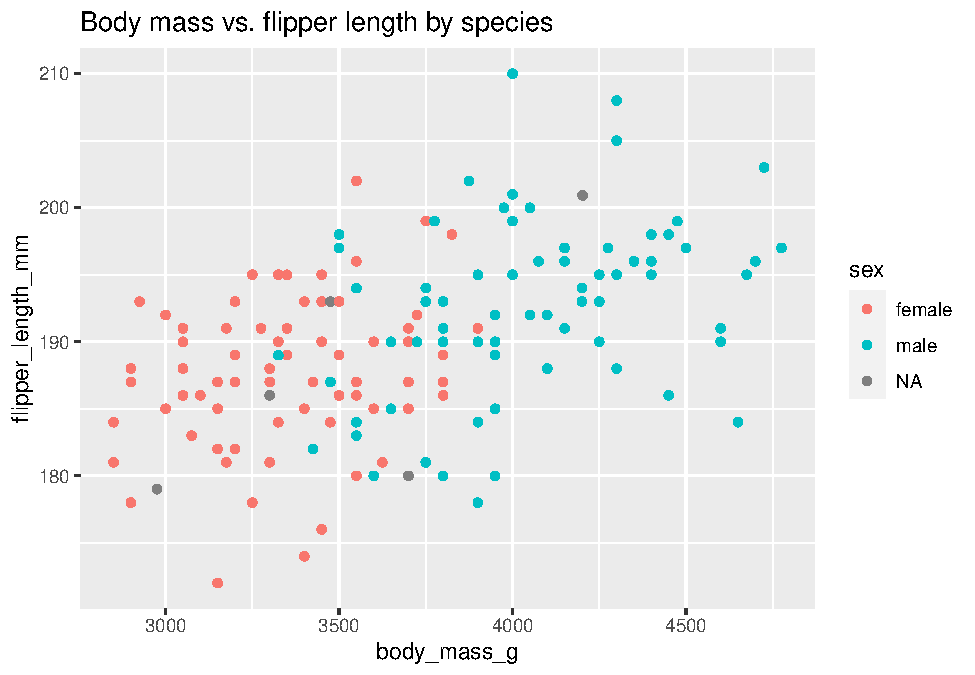
\includegraphics{data_files/figure-latex/unnamed-chunk-14-1.pdf}

\hypertarget{back-to-the-future}{%
\section{Back to the future}\label{back-to-the-future}}

Lets play a little more with grouping in the penguins dataset. Lets try
to ignore the missing values for now instead of imputing them.

\hypertarget{get-summary-of-a-statistic-but-grouping-on-another-variable}{%
\subsection{Get summary of a statistic, but grouping on another
variable}\label{get-summary-of-a-statistic-but-grouping-on-another-variable}}

\begin{Shaded}
\begin{Highlighting}[]
\NormalTok{penguins }\SpecialCharTok{\%\textgreater{}\%} 
  \FunctionTok{group\_by}\NormalTok{(species) }\SpecialCharTok{\%\textgreater{}\%}
  \FunctionTok{summarize}\NormalTok{(}
    \AttributeTok{mean\_bm =}\FunctionTok{mean}\NormalTok{(body\_mass\_g, }\AttributeTok{na.rm=}\NormalTok{T),}
    \AttributeTok{sd\_bm   =}\FunctionTok{sd}\NormalTok{(body\_mass\_g, }\AttributeTok{na.rm=}\NormalTok{T),}
    \AttributeTok{n            =} \FunctionTok{n}\NormalTok{()}
\NormalTok{)}
\end{Highlighting}
\end{Shaded}

\begin{verbatim}
## # A tibble: 3 x 4
##   species   mean_bm sd_bm     n
##   <fct>       <dbl> <dbl> <int>
## 1 Adelie      3701.  459.   152
## 2 Chinstrap   3733.  384.    68
## 3 Gentoo      5076.  504.   124
\end{verbatim}

\hypertarget{grouping-on-more-than-one-variable}{%
\subsection{Grouping on more than one
variable}\label{grouping-on-more-than-one-variable}}

\begin{Shaded}
\begin{Highlighting}[]
\NormalTok{penguins }\SpecialCharTok{\%\textgreater{}\%} 
  \FunctionTok{group\_by}\NormalTok{(species, sex) }\SpecialCharTok{\%\textgreater{}\%}
  \FunctionTok{summarize}\NormalTok{(}
    \AttributeTok{mean\_bm =}\FunctionTok{mean}\NormalTok{(body\_mass\_g, }\AttributeTok{na.rm=}\NormalTok{T),}
    \AttributeTok{sd\_bm   =}\FunctionTok{sd}\NormalTok{(body\_mass\_g, }\AttributeTok{na.rm=}\NormalTok{T),}
    \AttributeTok{n            =} \FunctionTok{n}\NormalTok{()}
\NormalTok{)}
\end{Highlighting}
\end{Shaded}

\begin{verbatim}
## `summarise()` has grouped output by 'species'. You can override using the
## `.groups` argument.
\end{verbatim}

\begin{verbatim}
## # A tibble: 8 x 5
## # Groups:   species [3]
##   species   sex    mean_bm sd_bm     n
##   <fct>     <fct>    <dbl> <dbl> <int>
## 1 Adelie    female   3369.  269.    73
## 2 Adelie    male     4043.  347.    73
## 3 Adelie    <NA>     3540   477.     6
## 4 Chinstrap female   3527.  285.    34
## 5 Chinstrap male     3939.  362.    34
## 6 Gentoo    female   4680.  282.    58
## 7 Gentoo    male     5485.  313.    61
## 8 Gentoo    <NA>     4588.  338.     5
\end{verbatim}

\hypertarget{remove-nas-sex-variable-and-sort-by-mean-body-size}{%
\subsection{Remove NAs sex variable and sort by mean body
size}\label{remove-nas-sex-variable-and-sort-by-mean-body-size}}

\begin{Shaded}
\begin{Highlighting}[]
\NormalTok{penguins }\SpecialCharTok{\%\textgreater{}\%} 
  \FunctionTok{filter}\NormalTok{(}\SpecialCharTok{!}\FunctionTok{is.na}\NormalTok{(sex)) }\SpecialCharTok{\%\textgreater{}\%} 
  \FunctionTok{group\_by}\NormalTok{(species, sex) }\SpecialCharTok{\%\textgreater{}\%}
  \FunctionTok{summarize}\NormalTok{(}
    \AttributeTok{mean\_bm =}\FunctionTok{mean}\NormalTok{(body\_mass\_g, }\AttributeTok{na.rm=}\NormalTok{T),}
    \AttributeTok{sd\_bm   =}\FunctionTok{sd}\NormalTok{(body\_mass\_g, }\AttributeTok{na.rm=}\NormalTok{T),}
    \AttributeTok{n            =} \FunctionTok{n}\NormalTok{()}
\NormalTok{)}\SpecialCharTok{\%\textgreater{}\%} 
\FunctionTok{arrange}\NormalTok{(}\FunctionTok{desc}\NormalTok{(mean\_bm))}
\end{Highlighting}
\end{Shaded}

\begin{verbatim}
## `summarise()` has grouped output by 'species'. You can override using the
## `.groups` argument.
\end{verbatim}

\begin{verbatim}
## # A tibble: 6 x 5
## # Groups:   species [3]
##   species   sex    mean_bm sd_bm     n
##   <fct>     <fct>    <dbl> <dbl> <int>
## 1 Gentoo    male     5485.  313.    61
## 2 Gentoo    female   4680.  282.    58
## 3 Adelie    male     4043.  347.    73
## 4 Chinstrap male     3939.  362.    34
## 5 Chinstrap female   3527.  285.    34
## 6 Adelie    female   3369.  269.    73
\end{verbatim}

Great! That was the fast introduction to penguins. Think about what you
learned from this. \textbf{The meta-information that you gather from
doing exercises as the ones above is the real magic}. Therefore, as
always, look at your data in different ways before diving in.

\hypertarget{lets-look-at-a-dataset-from-the-internet}{%
\section{Lets look at a dataset from the
internet}\label{lets-look-at-a-dataset-from-the-internet}}

Open this link in a new tab by copy-pasting and save it to your computer
using right-click
(\url{https://raw.githubusercontent.com/zief0002/miniature-garbanzo/main/data/gapminder.csv}).
Save it as ``gapminder2017''.

\hypertarget{comma-separated-csv}{%
\subsection{comma separated (csv)}\label{comma-separated-csv}}

try reading it in using read csv, the file ending is automatically put
on there, so even though you did not name it gapminder2017.csv, that is
the name it will get.

\begin{Shaded}
\begin{Highlighting}[]
\CommentTok{\# read csv can create in comma{-}separated files, read.table can be used to read in tab separated tables}
\CommentTok{\# BUT in general, you just need to specify what separated your columns and if the data has a header}
\NormalTok{gapminder2017 }\OtherTok{\textless{}{-}}\FunctionTok{read.csv}\NormalTok{(}\StringTok{"\textasciitilde{}/241023\_phdcourse/data/gapminder2017.csv"}\NormalTok{)}

\FunctionTok{glimpse}\NormalTok{(gapminder2017)}
\end{Highlighting}
\end{Shaded}

\begin{verbatim}
## Rows: 193
## Columns: 8
## $ country      <chr> "Afghanistan", "Albania", "Algeria", "Andorra", "Angola",~
## $ region       <chr> "Asia", "Europe", "Africa", "Europe", "Africa", "Americas~
## $ income       <dbl> 2.03, 13.30, 11.60, 58.30, 6.93, 21.00, 22.70, 12.70, 49.~
## $ income_level <chr> "Level 1", "Level 3", "Level 3", "Level 4", "Level 2", "L~
## $ life_exp     <dbl> 62.7, 78.4, 76.0, 82.1, 64.6, 76.2, 76.5, 75.6, 82.9, 82.~
## $ co2          <dbl> 0.254, 1.590, 3.690, 6.120, 1.120, 5.880, 4.410, 1.890, 1~
## $ co2_change   <chr> "increase", "increase", "increase", "decrease", "decrease~
## $ population   <dbl> 37.2000, 2.8800, 42.2000, 0.0770, 30.8000, 0.0963, 44.400~
\end{verbatim}

Plotting is useful for understanding your data, in this case, we can
plot the life expectancy and co2 across regions. We will back to
plotting much more so dont worry if you dont understand it all right
now.

\begin{Shaded}
\begin{Highlighting}[]
\FunctionTok{ggplot}\NormalTok{(gapminder2017, }\FunctionTok{aes}\NormalTok{(}\AttributeTok{x =}\NormalTok{ life\_exp, }\AttributeTok{y =}\NormalTok{ co2, }\AttributeTok{color =}\NormalTok{ region)) }\SpecialCharTok{+}
  \FunctionTok{geom\_point}\NormalTok{() }\SpecialCharTok{+}  \CommentTok{\# Add points for each data point}
  \FunctionTok{geom\_smooth}\NormalTok{(}\AttributeTok{method =} \StringTok{"lm"}\NormalTok{, }\AttributeTok{se =} \ConstantTok{FALSE}\NormalTok{) }\SpecialCharTok{+}  \CommentTok{\# Add linear trendlines without confidence bands}
  \FunctionTok{labs}\NormalTok{(}\AttributeTok{title =} \StringTok{"Life Expectancy vs. CO2 Levels across Regions (2017)"}\NormalTok{, }\AttributeTok{x =} \StringTok{"CO2 Levels"}\NormalTok{, }\AttributeTok{y =} \StringTok{"Life Expectancy"}\NormalTok{)}
\end{Highlighting}
\end{Shaded}

\begin{verbatim}
## `geom_smooth()` using formula = 'y ~ x'
\end{verbatim}

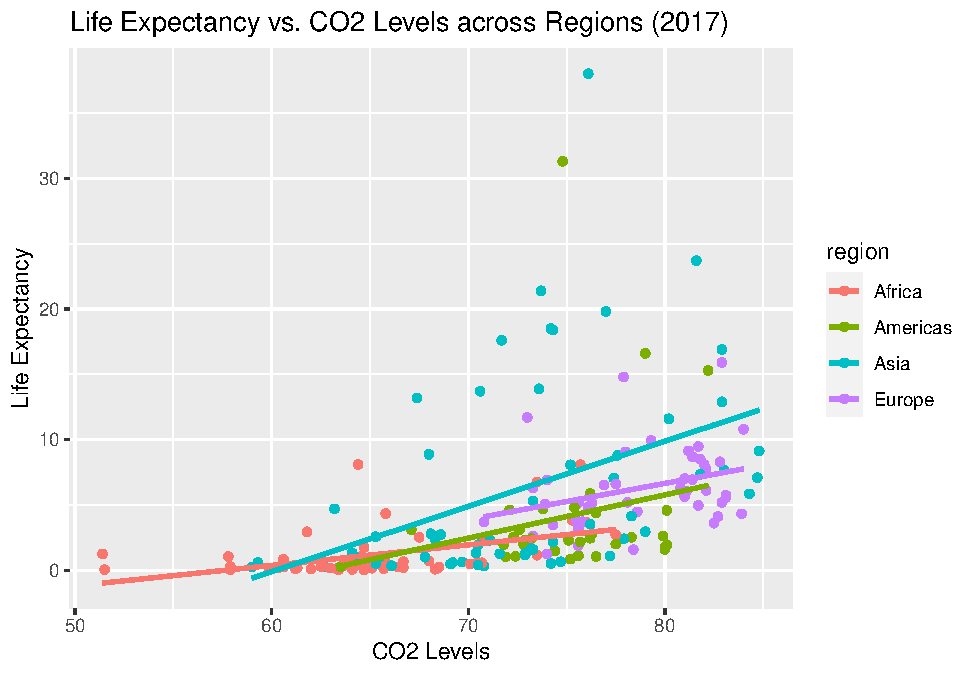
\includegraphics{data_files/figure-latex/unnamed-chunk-20-1.pdf}

However, what we want is not a point estimate for the year 2017, we want
the change in life expectancy over time across regions, but not per
year. We want to do it per 5 years to remove the uncertainty given by
yearly measurements also we only want to look at the Nordic countries.
The full dataset for gapminder is available in the R package
\texttt{gapminder} install this if you have not done so already.

For an overview of the data, look at this plot

\begin{Shaded}
\begin{Highlighting}[]
\FunctionTok{library}\NormalTok{(gapminder)}

\CommentTok{\# For Denmark see the trend in life expectancy}
\NormalTok{gapminder }\SpecialCharTok{\%\textgreater{}\%} \FunctionTok{filter}\NormalTok{(continent }\SpecialCharTok{\%in\%} \StringTok{"Europe"}\NormalTok{) }\SpecialCharTok{\%\textgreater{}\%} 
  \FunctionTok{ggplot}\NormalTok{(., }\FunctionTok{aes}\NormalTok{(}\AttributeTok{x =}\NormalTok{ year, }\AttributeTok{y =}\NormalTok{ lifeExp, }\AttributeTok{color =}\NormalTok{ country)) }\SpecialCharTok{+}
  \FunctionTok{geom\_point}\NormalTok{() }\SpecialCharTok{+}
  \FunctionTok{geom\_smooth}\NormalTok{(}\AttributeTok{method =} \StringTok{"lm"}\NormalTok{, }\AttributeTok{se =} \ConstantTok{FALSE}\NormalTok{)  }\CommentTok{\# Add linear trendlines without confidence bands}
\end{Highlighting}
\end{Shaded}

\begin{verbatim}
## `geom_smooth()` using formula = 'y ~ x'
\end{verbatim}

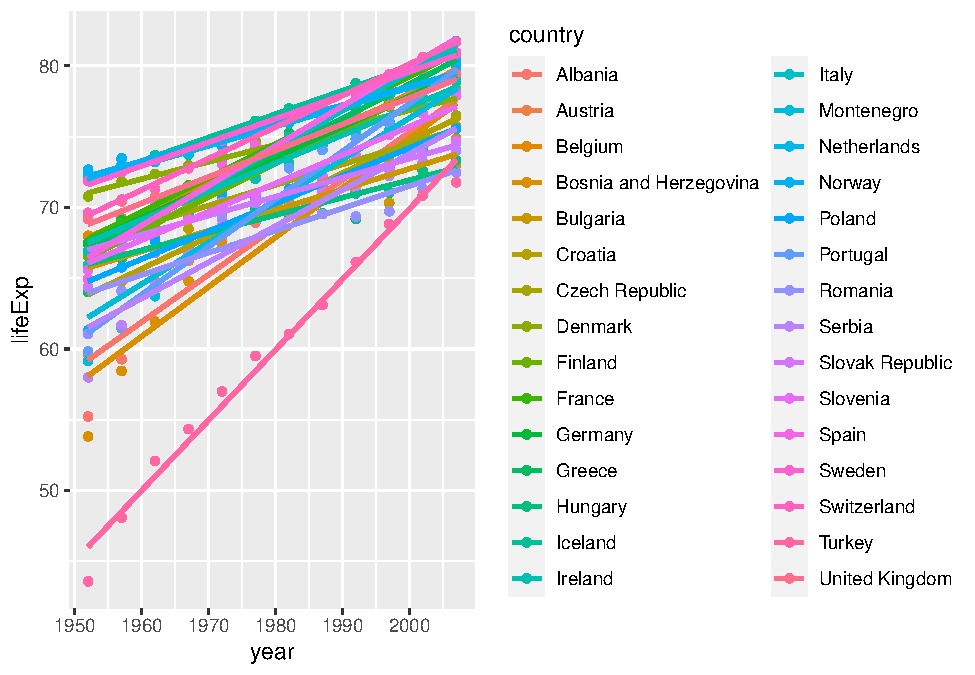
\includegraphics{data_files/figure-latex/unnamed-chunk-21-1.pdf}

\hypertarget{construct-new-date-variable-and-look-at-life-expectancy}{%
\subsection{Construct new date variable and look at life
expectancy}\label{construct-new-date-variable-and-look-at-life-expectancy}}

Often, we are given raw data and we need to invent a new feature that
incorporates the flaws of our data while still being useful. For
example, yearly estimates might not be available and thus we want to
contruct a 5 year period increase to remove some of uncertainty
introduced by this effect.

\begin{Shaded}
\begin{Highlighting}[]
\CommentTok{\# Filter data for Nordic countries in the \textquotesingle{}gapminder\textquotesingle{} dataset}
\NormalTok{nordic\_countries }\OtherTok{\textless{}{-}} \FunctionTok{c}\NormalTok{(}\StringTok{"Denmark"}\NormalTok{, }\StringTok{"Finland"}\NormalTok{, }\StringTok{"Iceland"}\NormalTok{, }\StringTok{"Norway"}\NormalTok{, }\StringTok{"Sweden"}\NormalTok{)}
\NormalTok{nordic\_data }\OtherTok{\textless{}{-}}\NormalTok{ gapminder }\SpecialCharTok{\%\textgreater{}\%} \FunctionTok{filter}\NormalTok{(country }\SpecialCharTok{\%in\%}\NormalTok{ nordic\_countries)}

\CommentTok{\# Create a date interval of five years}
\NormalTok{nordic\_data }\OtherTok{\textless{}{-}}\NormalTok{ nordic\_data }\SpecialCharTok{\%\textgreater{}\%}
  \FunctionTok{mutate}\NormalTok{(}\AttributeTok{year\_interval =}\NormalTok{ year }\SpecialCharTok{\%/\%} \DecValTok{5} \SpecialCharTok{*} \DecValTok{5}\NormalTok{)  }\CommentTok{\# Create intervals of 5 years}

\CommentTok{\# Summarize life expectancy for the Nordic countries within the 5{-}year intervals}
\NormalTok{summary }\OtherTok{\textless{}{-}}\NormalTok{ nordic\_data }\SpecialCharTok{\%\textgreater{}\%}
  \FunctionTok{group\_by}\NormalTok{(country, year\_interval) }\SpecialCharTok{\%\textgreater{}\%}
  \FunctionTok{summarise}\NormalTok{(}\AttributeTok{avg\_life\_expectancy =} \FunctionTok{mean}\NormalTok{(lifeExp, }\AttributeTok{na.rm =} \ConstantTok{TRUE}\NormalTok{))}
\end{Highlighting}
\end{Shaded}

\begin{verbatim}
## `summarise()` has grouped output by 'country'. You can override using the
## `.groups` argument.
\end{verbatim}

\begin{Shaded}
\begin{Highlighting}[]
\CommentTok{\# Show the summarized data}
\NormalTok{summary}
\end{Highlighting}
\end{Shaded}

\begin{verbatim}
## # A tibble: 60 x 3
## # Groups:   country [5]
##    country year_interval avg_life_expectancy
##    <fct>           <dbl>               <dbl>
##  1 Denmark          1950                70.8
##  2 Denmark          1955                71.8
##  3 Denmark          1960                72.4
##  4 Denmark          1965                73.0
##  5 Denmark          1970                73.5
##  6 Denmark          1975                74.7
##  7 Denmark          1980                74.6
##  8 Denmark          1985                74.8
##  9 Denmark          1990                75.3
## 10 Denmark          1995                76.1
## # i 50 more rows
\end{verbatim}

\begin{Shaded}
\begin{Highlighting}[]
\FunctionTok{ggplot}\NormalTok{(summary, }\FunctionTok{aes}\NormalTok{(}\AttributeTok{x =} \FunctionTok{factor}\NormalTok{(year\_interval), }\AttributeTok{y =}\NormalTok{ avg\_life\_expectancy, }\AttributeTok{fill =}\NormalTok{ country)) }\SpecialCharTok{+}
  \FunctionTok{geom\_bar}\NormalTok{(}\AttributeTok{stat =} \StringTok{"identity"}\NormalTok{, }\AttributeTok{position =} \StringTok{"dodge"}\NormalTok{) }\SpecialCharTok{+}
  \FunctionTok{labs}\NormalTok{(}\AttributeTok{title =} \StringTok{"Average Life Expectancy of Nordic Countries by 5{-}Year Intervals"}\NormalTok{, }\AttributeTok{x =} \StringTok{"Year Interval"}\NormalTok{, }\AttributeTok{y =} \StringTok{"Average Life Expectancy"}\NormalTok{) }\SpecialCharTok{+}
  \FunctionTok{scale\_fill\_brewer}\NormalTok{(}\AttributeTok{palette =} \StringTok{"Set1"}\NormalTok{)  }\CommentTok{\# Adjust the color palette as desired}
\end{Highlighting}
\end{Shaded}

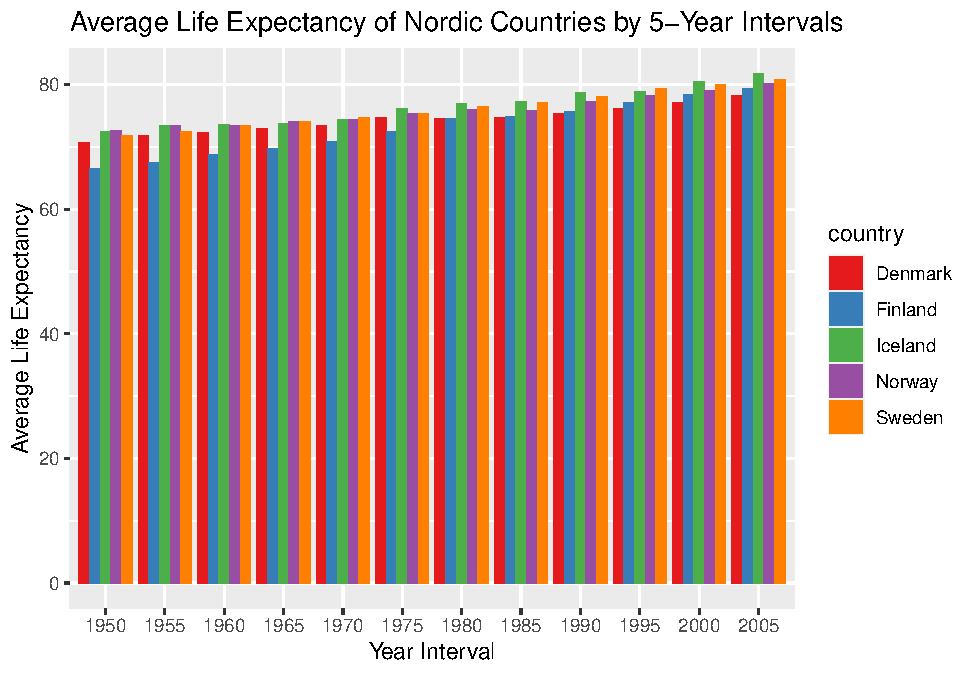
\includegraphics{data_files/figure-latex/unnamed-chunk-22-1.pdf}

\hypertarget{your-turn-1}{%
\subsection{Your turn}\label{your-turn-1}}

Exercise 4.

Now using the dataset \textbf{summary} we want to see how the
percentwise increase between 1950 and year 2005 differs between the
Nordic countries

\begin{enumerate}
\def\labelenumi{\arabic{enumi}.}
\tightlist
\item
  Create a new dataframe which contains the relative increase in life
  expectancy across Nordic countries between years and arrange from
  highest to lowest
\end{enumerate}

\backmatter
\end{document}
